%%%%%%%%%%%%%%%%%%%%%%%%%%%%%%%%%%%%%%%%%%%%%%%%%%%%%%%%%%%%%%%%%%%%%%
% LaTeX Example: Project Report
%
% Source: http://www.howtotex.com
%
% Feel free to distribute this example, but please keep the referral
% to howtotex.com
% Date: March 2011 
% 
%%%%%%%%%%%%%%%%%%%%%%%%%%%%%%%%%%%%%%%%%%%%%%%%%%%%%%%%%%%%%%%%%%%%%%
% How to use writeLaTeX: 
%
% You edit the source code here on the left, and the preview on the
% right shows you the result within a few seconds.
%
% Bookmark this page and share the URL with your co-authors. They can
% edit at the same time!
%
% You can upload figures, bibliographies, custom classes and
% styles using the files menu.
%
% If you're new to LaTeX, the wikibook is a great place to start:
% http://en.wikibooks.org/wiki/LaTeX
%
%%%%%%%%%%%%%%%%%%%%%%%%%%%%%%%%%%%%%%%%%%%%%%%%%%%%%%%%%%%%%%%%%%%%%%
% Edit the title below to update the display in My Documents
%\title{Project Report}
%
%%% Preamble
\documentclass[paper=a4, fontsize=11pt, bibliography=totocnumbered]{scrartcl}
\usepackage[T1]{fontenc}
\usepackage{fourier}

\usepackage[english]{babel}	% English language/hyphenation
\usepackage[protrusion=true,expansion=true]{microtype}	
\usepackage{amsmath,amsfonts,amsthm} % Math packages
\usepackage[pdftex]{graphicx}
\usepackage{float}
\usepackage{url}
\graphicspath{{images/}}
\usepackage{wrapfig}
\usepackage{todonotes}
\usepackage{array}
\usepackage{cleveref}
\usepackage{csquotes}% Recommended

\usepackage[style=ieee,backend=biber,urldate=iso8601,date=iso8601]{biblatex}

\addbibresource{references.bib}
\urlstyle{same}
\renewcommand*{\bibfont}{\small}

%%% Custom sectioning
\usepackage{sectsty}
\allsectionsfont{\normalfont\scshape}

\makeatletter
\renewcommand\paragraph{\@startsection{paragraph}{4}{\z@}%
  {-3.25ex \@plus -1ex \@minus -0.2ex}%
  {0.01pt}%
  {\raggedsection\normalfont\sectfont\nobreak\size@paragraph}%
}
\makeatother

\usepackage{scrlayer-scrpage}
\cfoot{\pagemark}

\usepackage[toc,section,numberedsection=autolabel,xindy]{glossaries}

\newglossaryentry{api}
{
    name={API},
    description={An \glsentryfirst{api} is a particular set
            of rules and specifications that a software program can follow to access and make use of the services and resources provided by another particular software program that implements that API},
    first={\glsentrylong{api}} (\glsentryname{api}),
    long={Application Programming Interface}
}

\newglossaryentry{poets}
{
	name={POETS},
    description={\glsentryfirst{poets} is a system based around many simple computation cores running at the same time that communicate with simple messages},
    first={\glsentrylong{poets}} (\glsentryname{poets}),
    long={Partial Ordered Event Triggered Systems}
}

\newglossaryentry{software node}
{
	name={software node},
    description={A software node is a single point in the overall \gls{poets} graph. It consists of a single receive, send and compute handler and acts as a destination and/or source for messages. A \gls{poets} system is composed of multiple nodes although multiple nodes can run on a single hardware instance such a \gls{cpu}}
}

\newglossaryentry{network node}
{
	name={network node},
    description={A network node is a physical entity that is part of a \todo{finish}}
}

\newglossaryentry{nios}
{
	name={NIOS},
    description={NIOS is a \gls{soft processor} architecture used by Altera to allow for a \gls{cpu} to be implemented an \gls{fpga}. It is a 16-bit architecture with low hardware and power costs}
}

\newglossaryentry{cpu}
{
	name={CPU},
    description={A \glsentryfirst{cpu} is the electronic circuitry within a computer that carries out the instructions of a computer program by performing the basic arithmetic, logical, control and input/output (I/O) operations specified by the instructions},
    first={\glsentrylong{cpu}} (\glsentryname{cpu}),
    long={Central Processing Unit}
}

\newglossaryentry{gpu}
{
	name={GPU},
    description={A \glsentryfirst{gpu} \todo{finish gpu description}},
    first={\glsentrylong{gpu}} (\glsentryname{gpu}),
    long={Graphics Processing Unit}
}

\newglossaryentry{fpga}
{
	name={FPGA},
    long={Field-Programmable Gate Array},
    first={\glsentrylong{fpga}} (\glsentryname{fpga}),
    description={A \glsentryfirst{fpga} is an integrated circuit designed to be configured by a customer or a designer after manufacturing}
}

\newglossaryentry{soft processor}
{
	name={soft microprocessor},
    description={A soft microprocessor (also called softcore microprocessor or a soft processor) is a microprocessor core that can be wholly implemented using logic synthesis}
}

\newglossaryentry{ide}
{
	name={IDE},
    long={Integrated Development Environment},
    description={An \glsentryfirst{ide} is a software application that provides comprehensive facilities to computer programmers for software development. An IDE normally consists of a source code editor, build automation tools and a debugger},
    first={\glsentrylong{ide}} (\glsentryname{ide})
}

\newglossaryentry{hls}
{
	name={HLS},
    long={High Level Synthesis},
    description={\glsentryfirst{hls}, is an automated design process that interprets an algorithmic description of a desired behaviour and creates digital hardware that implements that behaviour},
    first={\glsentrylong{hls}} (\glsentryname{hls})
}

\newglossaryentry{avalon}
{
	name={Avalon},
    description={\glsentryname{avalon} is an interface created by Altera for easy creation of complex digital systems. It supports high-speed data streaming as well as address based data access from memory or peripherals}
}

\newglossaryentry{thread}
{
	name={thread},
    description={A \glsentryname{thread} is a \todo{finish}}
}

\newglossaryentry{hal}
{
	name={HAL},
    long={Hardware Abstraction Layer},
    first={\glsentrylong{hal}} (\glsentryname{hal}),
    description={Nios II Hardware Abstraction Layer (HAL) is a well defined software layer that forms a clear distinction between application and device-level software. The HAL also provides services such as file descriptors, I/O control, and buffering, which are required by the ANSI C library functions\cite{wiki:hal}}
}

\newglossaryentry{os}
{
	name={OS},
    long={Operating System},
    first={\glsentrylong{os}} (\glsentryname{os}),
    description={An \glsentryfirst{os} is system software that manages computer hardware and software resources and provides common services for computer programs. All computer programs, excluding firmware, require an operating system to function}
}

\newglossaryentry{application}
{
	name={application},
    description={\todo{Make description}}
}

\newglossaryentry{bit-exact}
{
	name={bit-exact},
    description={\glsentryname{bit-exact} means that for two given pieces of data, when converted to a binary format are identical. Each bit of the first piece of data is exactly the same as the corresponding bit in the second piece of data}
}

\newglossaryentry{logic element}
{
	name={logic element},
    description={\todo{describe}}
}

\newglossaryentry{port}
{
	name={port},
    description={\todo{description}}
}

\newglossaryentry{edge}
{
	name={channel},
    description={\todo{describe}}
}

\newglossaryentry{source port}
{
	name={source port},
    description={\todo{describe}}
}

\newglossaryentry{destination port}
{
	name={destination port},
    description={\todo{describe}}
}

\newglossaryentry{message}
{
	name={message},
    description={\todo{describe}}
}

\newglossaryentry{tcp}
{
	name={TCP},
    long={Transmission Control Protocol},
    first={\glsentrylong{tcp}} (\glsentryname{tcp}),
    description={\glsentryname{tcp} is a standard that defines how to establish and maintain a network conversation via which application programs can exchange data.It  enables two hosts to establish a connection and exchange streams of data. \glsentryname{tcp} guarantees delivery of data and also guarantees that packets will be delivered in the same order in which they were sent}
}

\newglossaryentry{spinnaker}
{
	name={SpiNNaker},
    long={Spiking Neural Network Architecture},
    first={\glsentrylong{spinnaker}} (\glsentryname{spinnaker}),
    description={\todo{describe}}
}

\newglossaryentry{gals}
{
	name={GALS},
    long={Globally Asynchronous, Locally Synchronous},
    first={\glsentrylong{gals}} (\glsentryname{gals}),
    description={\todo{describe}}
}

\newglossaryentry{sdram}
{
	name={SDRAM},
    description={\todo{describe}}
}

\newglossaryentry{soc}
{
	name={SoC},
    long={System on a Chip},
    description={\todo{describe}},
    first={\glsentrylong{soc}} (\glsentryname{soc})
}

\newglossaryentry{fifo}
{
	name={FIFO},
    long={First In, First Out},
    first={\glsentrylong{fifo}} (\glsentryname{fifo}),
    description={A \glsentryfirst{fifo} buffer or queue is a type of buffer that uses the First In, First Out procedure. When data is added to it, it is put on the back of the existing data and when data is removed, the data comes from the front of the stored data}
}

\newglossaryentry{quartus}
{
	name={Quartus},
    description={\todo[inline]{Write description}}
}

\newglossaryentry{noc}
{
	name={NoC},
    long={Network on a Chip},
    first={\glsentrylong{noc}} (\glsentryname{noc}),
    description ={\todo{Describe}}
}

\newglossaryentry{dircc}
{
	name={DiRCC},
    long={Distributed Reconfigurable Cloud Computing},
    first={\glsentrylong{dircc}} (\glsentryname{dircc}),
    description={\todo{describe}}
}
\makeglossaries

\renewcommand{\glstextformat}[1]{\textit{#1}}

%%% Equation and float numbering
\numberwithin{equation}{section}		% Equationnumbering: section.eq#
\numberwithin{figure}{section}			% Figurenumbering: section.fig#
\numberwithin{table}{section}				% Tablenumbering: section.tab#


%%% Maketitle metadata
\newcommand{\horrule}[1]{\rule{\linewidth}{#1}} 	% Horizontal rule

\title{
		%\vspace{-1in} 	
		\usefont{OT1}{bch}{b}{n}
		\normalfont \normalsize \textsc{Imperial College, London} \\ [25pt]
		\horrule{0.5pt} \\[0.4cm]
		\huge Interim Report \\
		\horrule{2pt} \\[0.5cm]
}
\author{
		\normalfont 								\normalsize
        Patrick Engelbert \\[-3pt]		\normalsize
        \today
}
\date{} % Remove date here

%%% Begin document
\begin{document}
\maketitle

\clearpage

\tableofcontents

\clearpage

\section{Introduction}

Modern datacenters are starting to struggle to balance the requirements of high capacity computation with the ease of manageability, which together with the decreasing rate of \gls{cpu} improvements have caused datacenter providers to look towards \glspl{fpga} as a means of providing large scale reconfigurable computation for cloud based applications\cite{pub:configurable-cloud-acceleration}. 

Traditionally, cloud-based systems require a layer of abstraction between the physical hardware and the user application, both to effectively use all of the hardware without the user noticing and to provide isolation between the applications of multiple users. In this sense, running on \glspl{fpga} is no different and requires a layer of abstraction between the hardware and the applications.

With \gls{dircc}, the aim is to create a layer of abstraction between the \gls{fpga} hardware and the application that is running on top of it. To use the \gls{fpga} to it's fullest potential, the project is designed around small asynchronous computation nodes that are interconnected by a network to allow them to communicate and perform large and complex tasks by splitting them into many smaller manageable components that can be computed in parallel.

\section{Project Description}

Currently in development is the \gls{poets} project at Southampton University, Imperial College, London and other institutions. \Gls{poets} is designed as a system to provide distributed asynchronous computing using interconnected \glspl{cpu}. In essence, it has the same aim as \gls{dircc} except to run on a \gls{cpu} based architecture opposed to an \gls{fpga} based architecture.

To ease the development of \gls{dircc}, much of the specification is based on the specification of \gls{poets}, allowing for interoperability as well as the sharing of ideas between the two projects as well as providing a better abstraction layer that allows the \gls{application} code to be platform agnostic.

\subsection{\glsentryname{poets} Description}

\gls{poets} is a software infrastructure project which uses many small \glspl{software node} to break apart computation of time expensive and complex tasks into many smaller computations that all run at the same time and interact with each other through small \glspl{message}. On receiving such a \gls{message}, a handler is executed on the receiving \gls{software node}, potentially changing it's state and/or sending more \glspl{message}. All of the \glspl{software node} have a defined set of input and output \glspl{port} which provide a way to logically connect up multiple \glspl{software node} within the \gls{application}. These \glspl{port} are connected via \glspl{edge} which can be seen as a direct link between a \gls{source port} on one \gls{software node} and one \gls{destination port} on another \gls{software node} as shown in \cref{fig:poets_system}.

\begin{wrapfigure}{R}{0.6\textwidth}
\missingfigure{Missing Poets System}
\caption{System diagram of a simple POETS application}
\label{fig:poets_system}
\end{wrapfigure}

In addition, there is the possibility of attaching properties to \glspl{edge} which act as fixed data that is passed to the receiving \gls{software node}'s receive handler if the \gls{edge} with attached properties is the one that a \gls{message} has travelled along. For example, this would allow the receiving \glspl{software node} to know about sending \gls{software node}'s ID without this data having to be sent over the network.

As the \glspl{software node} are directly connected via \glspl{edge} (on the logical layer, although it may use a protocol like \gls{tcp} on the networking layer). This means that data is packaged into a \gls{message} automatically and the application does not need to worry about the source and destination \glspl{software node} as these are implicit in the system design. Due to the direct logical connection between two \glspl{software node}, \gls{poets} also guarantees that any \glspl{message} sent along an \gls{edge} will arrive at the destination \gls{software node} although due to the abstraction away from the hardware layer, it is unable to guarantee the order in which \glspl{message} will arrive at the destination \gls{software node}.

\paragraph{\Gls{poets} specification}

The following \gls{poets} requirements are applicable to \gls{dircc}.
\todo[inline]{Finish}
\begin{itemize}
\item POETS Spec 1
\item POETS Spec 2
\end{itemize}

\subsection{\Gls{dircc} Project Description}

\Gls{dircc} is a project that will be composed of the hardware in the form of \glspl{network node} and networking infrastructure, as well as the \gls{api} between this hardware and the \gls{poets} style application that will be running on it. To maintain compatibility with the \gls{poets} project, \gls{dircc} will be but around the same specifications, with only some minor changes to be compatible with \glspl{fpga}.

\todo[inline]{finish}
\begin{itemize}
\item DiRCC Spec 1
\end{itemize}

While in the ideal scenario, the system would be infinitely expandable, due to time and resource constraints, my project will be focussing on the generation of a system running on only a single \gls{fpga}. However, I will be taking into account the fact that the system may have to run, split over two or more \glspl{fpga} when designing it.

Similar projects have been done in the past such as Splash/Splash 2\cite{pub:1_arnold_buell_hoang_pryor_shirazi_thistle} or PRISM\cite{pub:agarwal1994asynchronous}. However, these projects tended to be aimed at either a very specific application, typically neural networks and machine learning or relied on custom hardware and would not be suitable for cloud based systems as shown in \cref{subsec:similar}. \Gls{dircc} however is aimed as a more generic system layer that has applications beyond those that comparative projects have, with a focus on large cloud scale systems.

In addition, with the recent completion of Project Catapult by Microsoft \cite{pub:configurable-cloud-acceleration} in which they added a single Stratix-V \gls{fpga} to each of the \glspl{cpu} for configurable computing in the cloud, it would be useful to re-purpose these \glspl{fpga} to act as a massive distributed network. In creating this project, the aim is ultimately allow developers to target only the \glspl{fpga} as the computational layer without requiring the \gls{cpu} at all.

\section{Background}

\subsection{Similar Research} 
\label{subsec:similar}

There are multiple projects focussed around event-based massively-parallel systems, on multiple \glspl{cpu} as well as \glspl{gpu} and even \glspl{fpga}. For the most part these systems are based around spiking neural network, in other words they are designed to mimic the precesses that the human brain uses, especially the connection of neurons and their interactions.

\todo[inline]{Update previous paragraph}

\paragraph{\glsentryname{spinnaker}} \label{subsec:spinnaker}

\begin{wrapfigure}{R}{0.4\textwidth}
\centering
\vspace{-\normalbaselineskip}
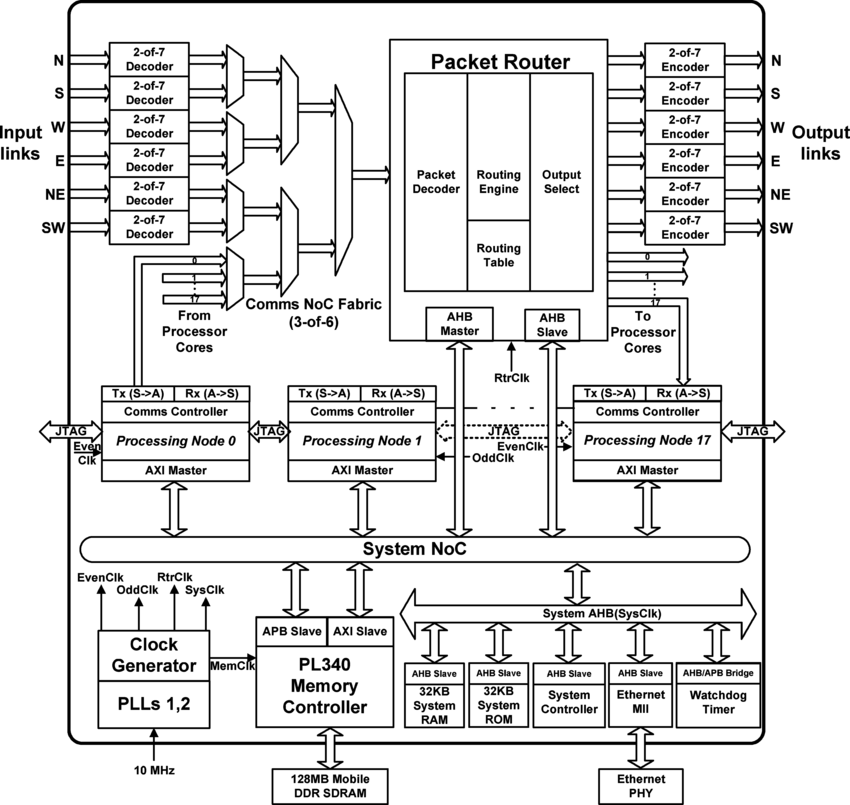
\includegraphics[width=0.35\textwidth,keepaspectratio]{Organization-of-the-SpiNNaker-CMP.png}
\caption{System diagram of a single \gls{spinnaker} node\cite{pub:painkras2012spinnaker}}
\label{fig:spinnaker_node}
\vspace{-\normalbaselineskip}
\end{wrapfigure}

The inspiration for the \gls{poets} project is a hardware design from The University of Manchester called \gls{spinnaker}\cite{pub:painkras2012spinnaker}. This is a system designed to model the actions of up to a billion neurons using up to 2\textsuperscript{16} software nodes connected together using an asynchronous network, allowing it to perform many calculations at the same time with \glspl{message} being passed between them. Due to the similarity between \gls{spinnaker} and \gls{dircc}, a large amount of the concepts of \gls{spinnaker} can be used as a starting point for it. Specifically, the details of the \gls{spinnaker} node and some of the routing infrastructure are of interest.

\Gls{spinnaker} is based around a large number of \gls{spinnaker} nodes that are all interconnected. Each of the nodes has two functions: they are the \glspl{cpu} that perform the actual communication, and include a router that forms the backbone of the network infrastructure. This means that for the \gls{spinnaker} system, these nodes must simply be connected together once when the hardware is built and the configuration can then be determined on the start of each program run without the hardware having to be changed. The design of the node is based around the \gls{gals} architecture\cite{art:1_plana_furber_temple_khan_shi_wu_yang_2007} to simplify timing closure in the \gls{soc} design and allow for redundancy within the node in case of a faulty processing node.

Each \gls{spinnaker} node is laid out as shown in \cref{fig:spinnaker_node} with 6 input and output links, an input clock, connection to some off-chip \gls{sdram}, an Ethernet interface to the external world and some JTAG interfaces to allow for debugging. \todo{expand}

Within each node, there are 18 ARM968 based Processor Nodes, of which one is chosen on start up as a monitor Processor Node to manage the other computing Processor Nodes and act as an interface to the external system with functions such as data aggregation. Each of these Processor Nodes is composed of an ARM9E-S integer core with attached 64KB of dual-banked data memory and 32KB of instruction memory as can e seen in \cref{fig:spinnaker_processor_node}. In addition, it has the typical timers and interrupt controllers as well as interfaces to the Processor Node's internal network.

All of Processor Nodes within a single \gls{spinnaker} node are connected to a networking infrastructure that attaches to the built-in \gls{message} router as well as a block of on-chip RAM, on-chip boot ROM and the off-chip \gls{sdram}. In addition, this networking layer connects to the interface for the Ethernet connection.
The second component of each \gls{spinnaker} node is the \gls{message} router. This component receives the \glspl{message} from all of the 6 input connections and decides into which of the output connections the \gls{message} should travel next. Alternative, the \gls{message} may have reached it's destination and so needs to be routed to the correct Processing Node. In addition, when a Processing Node wishes to send a \gls{message} to a different \gls{spinnaker} node, it too must travel through the router so that the correct output connection can be chosen.

The router is attached of several multiplexers to combine all of the possible input \gls{message} sources, whether on-chip or off-chip into a single \gls{message} stream that then feed into the input of the router. Within the router there are three pipeline stages to decode the message, decide on the route of the \gls{message} and push the \gls{message} into the appropriate output queue. In addition, there is a 1024 word routing table that is preloaded with the routing information at the application start\cite{pub:navaridas2009understanding}.

\begin{wrapfigure}{l}{0.4\textwidth}
\centering
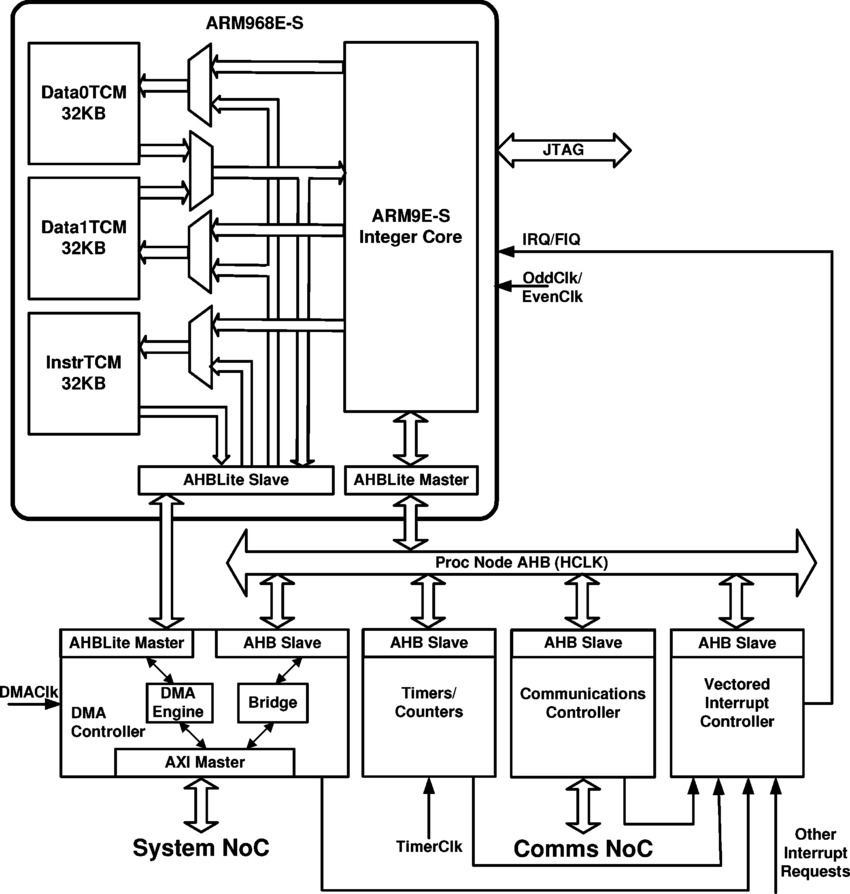
\includegraphics[width=0.35\textwidth,keepaspectratio]{Details-of-the-SpiNNaker-processor-node.png}
\caption{Details of a \gls{spinnaker} Processor Node\cite{pub:painkras2012spinnaker}}
\label{fig:spinnaker_processor_node}
\end{wrapfigure}

As can be seen in \cref{fig:gals_router}, once a \gls{message} has been decoded, there is an error checking stage that also steers the \gls{message} to the correct routing engine for the second stage. This second stage uses either a multicast router for, algorithmic router or point to point router to determine the next step that the \gls{message} should take\cite{art:1_plana_furber_temple_khan_shi_wu_yang_2007} based on both the message's source address as well as the data stored in the routing table. In the case of \gls{spinnaker}, the multicast router is the default choice for most \glspl{message} with point-to-point routing used as little as possible\cite{pub:navaridas2009understanding}. This is done to reduce the number of \glspl{message} that are traversing the network, especially if a large portion of the \glspl{message} travel the same path.

The second routing engine, the algorithmic routing, has two main modes. The first is called 'default routing'\cite{art:1_plana_furber_temple_khan_shi_wu_yang_2007} which occurs when the source address is not in the routing table and causes the \gls{message} to be passed to the opposite output connection, e.g. North to South. This saves space on the routing table and also reduces the complexity of the calculations required for most \glspl{message}. As such, it is a useful feature that should be included in the routing of \glspl{message} for my project as much as possible. The second mode for the algorithmic routing is one of neighbours, which routes the \gls{message} to all neighbours of the processing node. As this is heavily inspired by the way that synapses communicate, it is useful to the application that \gls{spinnaker} is designed for but is not too useful for my application.

The last routing engine, which is also the one most applicable to the one in this project, is the point-to-point routing. It is typically used for control \glspl{message} in the \gls{spinnaker} system but fits the description of the \gls{poets} system the closest.

The final part of the router is an emergency routing pipeline stage. When an output connection has been chosen, it attempts to send it along this path by placing it into a \gls{fifo} buffer to be sent as soon as it is ready. If this is not possible due to the buffer being full (thus the connection is congested) or if the connection is broken, the emergency routing is put in effect. In this case, the system routes the \gls{message} to one of it's neighbours to bypass the problem zone\cite{pub:navaridas2009understanding}. If this is not possible, the \gls{message} is dropped after a certain time to prevent deadlocks. While the dropping of \glspl{message} is not supported by \gls{poets}, the other aspects of the emergency routing is very much applicable to my project as it has the can have the same problems that will need to be overcome.

\begin{wrapfigure}{r}{0.4\textwidth}
\centering
\vspace{-\normalbaselineskip}
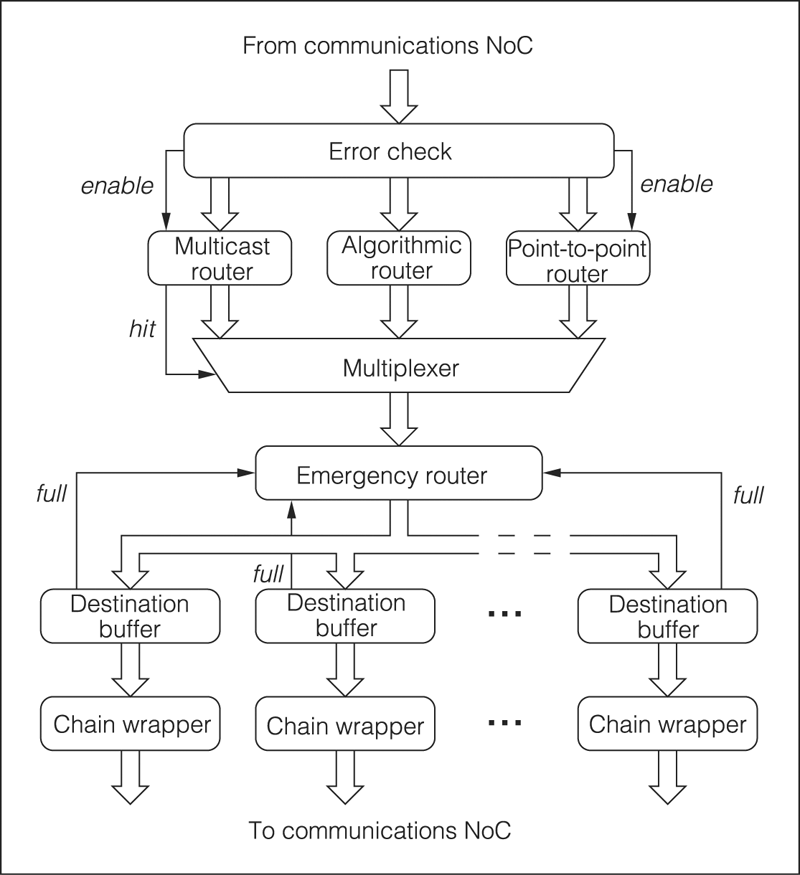
\includegraphics[width=0.35\textwidth,keepaspectratio]{gals_router.png}
\caption{Details of a \gls{gals} Router\cite{art:1_plana_furber_temple_khan_shi_wu_yang_2007}}
\label{fig:gals_router}
\end{wrapfigure}

One thing that the routing in \gls{spinnaker} does is manage the flow of \glspl{message} and congestion very well. Due to the nature of the default routing, most \glspl{message} travel along a straight line with at most a single point of inflection within it \cite{pub:2_khan_lester_plana_rast_jin_painkras_furber_2008}, thereby reducing congestion. In addition, this allows for a high throughput due to low processing cost as well as a lower memory requirements for the routing table.

As the \gls{spinnaker} project is very similar to this one, with the exception of the \gls{fpga} component, many of the design principles can be used as a starting point for this project. However, due to my project being an adaptation of \gls{poets} and designed for a broader range of applications than \gls{spinnaker} was, some of the design choices cannot be used while others must me modified to fit new criteria if they are to be taken into consideration.

\paragraph{PRISM}

Another similar project is PRISM\cite{pub:agarwal1994asynchronous} which is a small-scale proof of concept project for reconfigurable asynchronous computing. This project uses hardware based \glspl{cpu} with an attached \gls{fpga} for hardware acceleration of commonly executed instruction groups. However, it had issues due to the arbitrary nature of the application code, most noticeably the execution of loops and if/else code constructs on the \gls{fpga}.

\paragraph{Distributed \gls{fpga} Research Platform}

There is also a similar project at Bucknell University in 2011\cite{pub:2_su_2011} that attempted to provide a purely \gls{fpga} based distributed system for multiple application types. They were using a configuration with multiple \glspl{fpga}, each acting as a single \gls{software node} although the board I/O limited the performance gain that they could gain, especially for file heavy applications.

\subsection{Networking}

\begin{wrapfigure}{R}{0.6\textwidth}
\centering
\vspace{-2\normalbaselineskip}
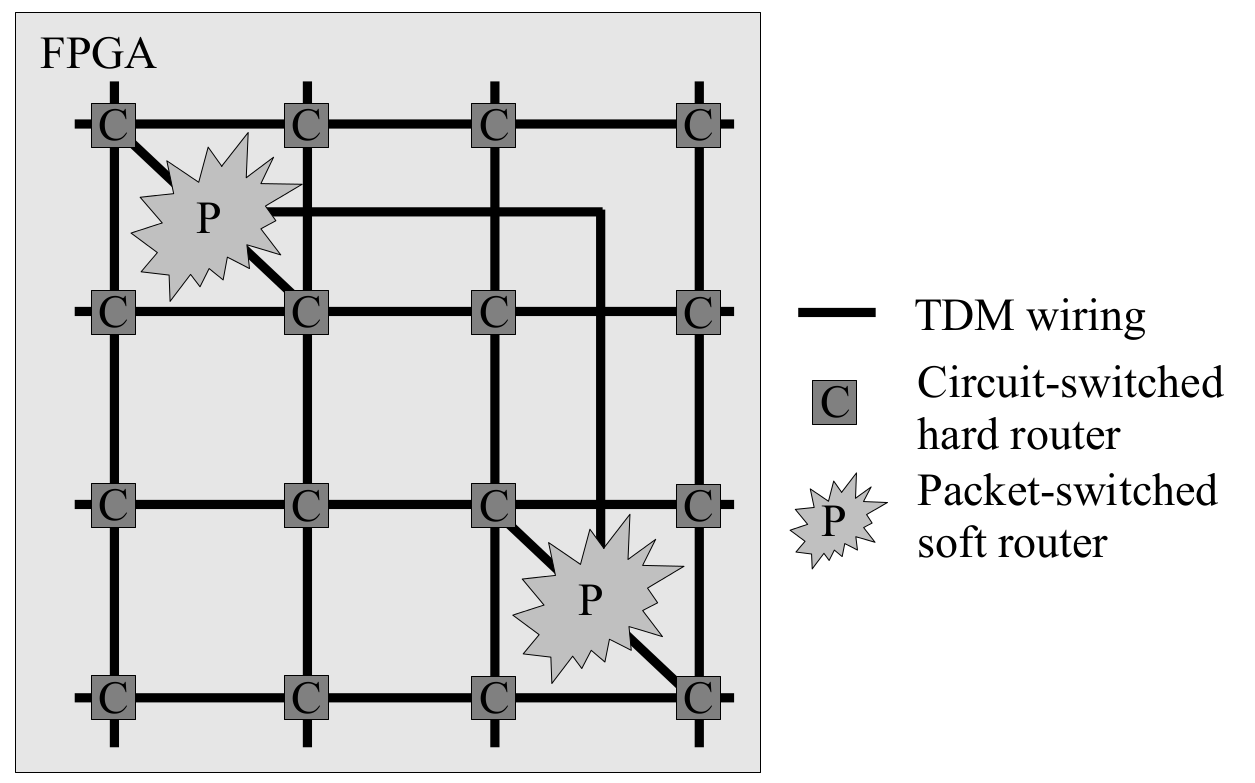
\includegraphics[width=0.55\textwidth,keepaspectratio]{switching_ucam.png}
\caption{Design of a circuit-switched local routing and message-switched distant routing\cite{rpt:francis2013exploring}}
\label{fig:francis_network}
\vspace{-\normalbaselineskip}
\end{wrapfigure}

According to R. Francis\cite{rpt:francis2013exploring}, an issue with for \gls{noc} on an \gls{fpga} is the difficulty of getting good latency without paying the price in terms of area. As such, she recommends a design that incorporates fast and low cost circuit switched \glspl{network node} for local networking with some \glspl{soft processor} as a message-switched routers for longer distance packages, reducing the latency of the number of hops that the \gls{message} would usually have to pass. This design also reduces the need for complex circuitry in the local circuit switched routers, while at the same time reduces the need for large look-up tables for distant destinations as shown in \cref{fig:francis_network}.

\subsection{Hardware}

\paragraph{\glsentrylong{fpga}}

To complete this project, an \gls{fpga} is required on which the project can be developed and evaluated. The main competitors in this category are the Xilinx Spartan series and Altera Cyclone series of \glspl{fpga}. Both are the low cost and low power \gls{fpga} categories from their respective companies and as such the ones that are most readily available.

Out of those two, the Altera Cyclone series of \glspl{fpga} is the more familiar require less time to develop on it. Within this series, the \glspl{fpga} that were readily available were the Cyclone III mounted on a Terasic DE0 board\cite{web:terasic_de0} and the Cyclone V mounted on a Terasic DE1-SoC board\cite{web:terasic_de1}. While both would have worked as an \gls{fpga} for this project, as the Cyclone V \gls{fpga} has a built in ARM Cortex-A9 processor and is supported by a newer version of the Quartus developments software, it is the better choice for \gls{dircc} development. While an older version of the development software would have been usable, the newer version, 16.1, has a better compiling and fitting algorithm built in which allows for faster and better optimised compilation compared to the older version, 13.1. Another major issue with the older version of the Quartus software is that it does not run on my machine, meaning that I have to either spend a large amount of time working around assorted compatibility bugs or find a different machine to work on.

In addition, the Altera Stratix V and Stratix X \glspl{fpga} are the ones targeted by the Microsoft \gls{fpga} cloud\cite{pub:configurable-cloud-acceleration} which are both supported on only the newest version of Quartus, with only the Stratix V being supported on older versions.

\begin{figure}
\centering
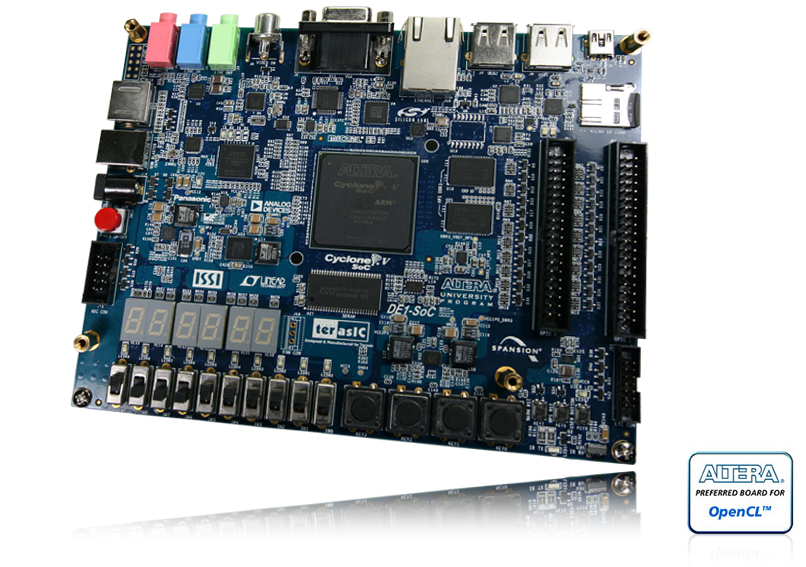
\includegraphics[width=0.35\textwidth,keepaspectratio]{DE1-SoC_top45_01.jpg}
\caption{Image of a DE1-SoC development board by Terasic\cite{img:terasic_fpga}}
\label{fig:de1}
\end{figure}

\section{Design}

\subsection{Design Decisions}

Based on the project requirements and the research of similar projects and components, a design similar to that of the \gls{spinnaker} project (\cref{subsec:spinnaker}) appears the most promising as the architecture and project requirements are very similar. Of course, some of the system will have differences due to \gls{dircc} being on an \gls{fpga} and so will have to be adapted.

Out of the available network architectures, the mesh-based network provides the best design in terms of redundancy, ease of creation and scaling at the expense of increasing the routing complexity and increased latency. However, the alternatives suggested by R. Francis\cite{rpt:francis2013exploring}, while useful, appear too complicated to implement properly in the time available. In addition, during this initial development of \gls{dircc}, it is unlikely that it will get large enough to warrant the long-range message-switched routing.

For the \glspl{network node}, the design will be in the form of a single \gls{software node} with attached memory and router. Initially, the \gls{software node} will run on a single \gls{nios} processor although these are expensive in area and have a low throughput so the aim, is to replace them with a custom Verilog block that is equivalent to the running \gls{poets} code without the need for a full \gls{soft processor} to run the code.

\subsection{Deliverables} \label{subsec:deliverables}

Based on the previous research and the project description, the following deliverables are required to deem the project a success.

\begin{itemize}\label{list:deliverables}
\item Create \gls{network node} design and implementation\todo{Reword all deliverables}
\item Create \gls{api} between the \glspl{network node} and \glspl{software node}
\end{itemize}

\section{Project Plan}

\subsection{Timeline}

\begin{figure}[H]
\centering
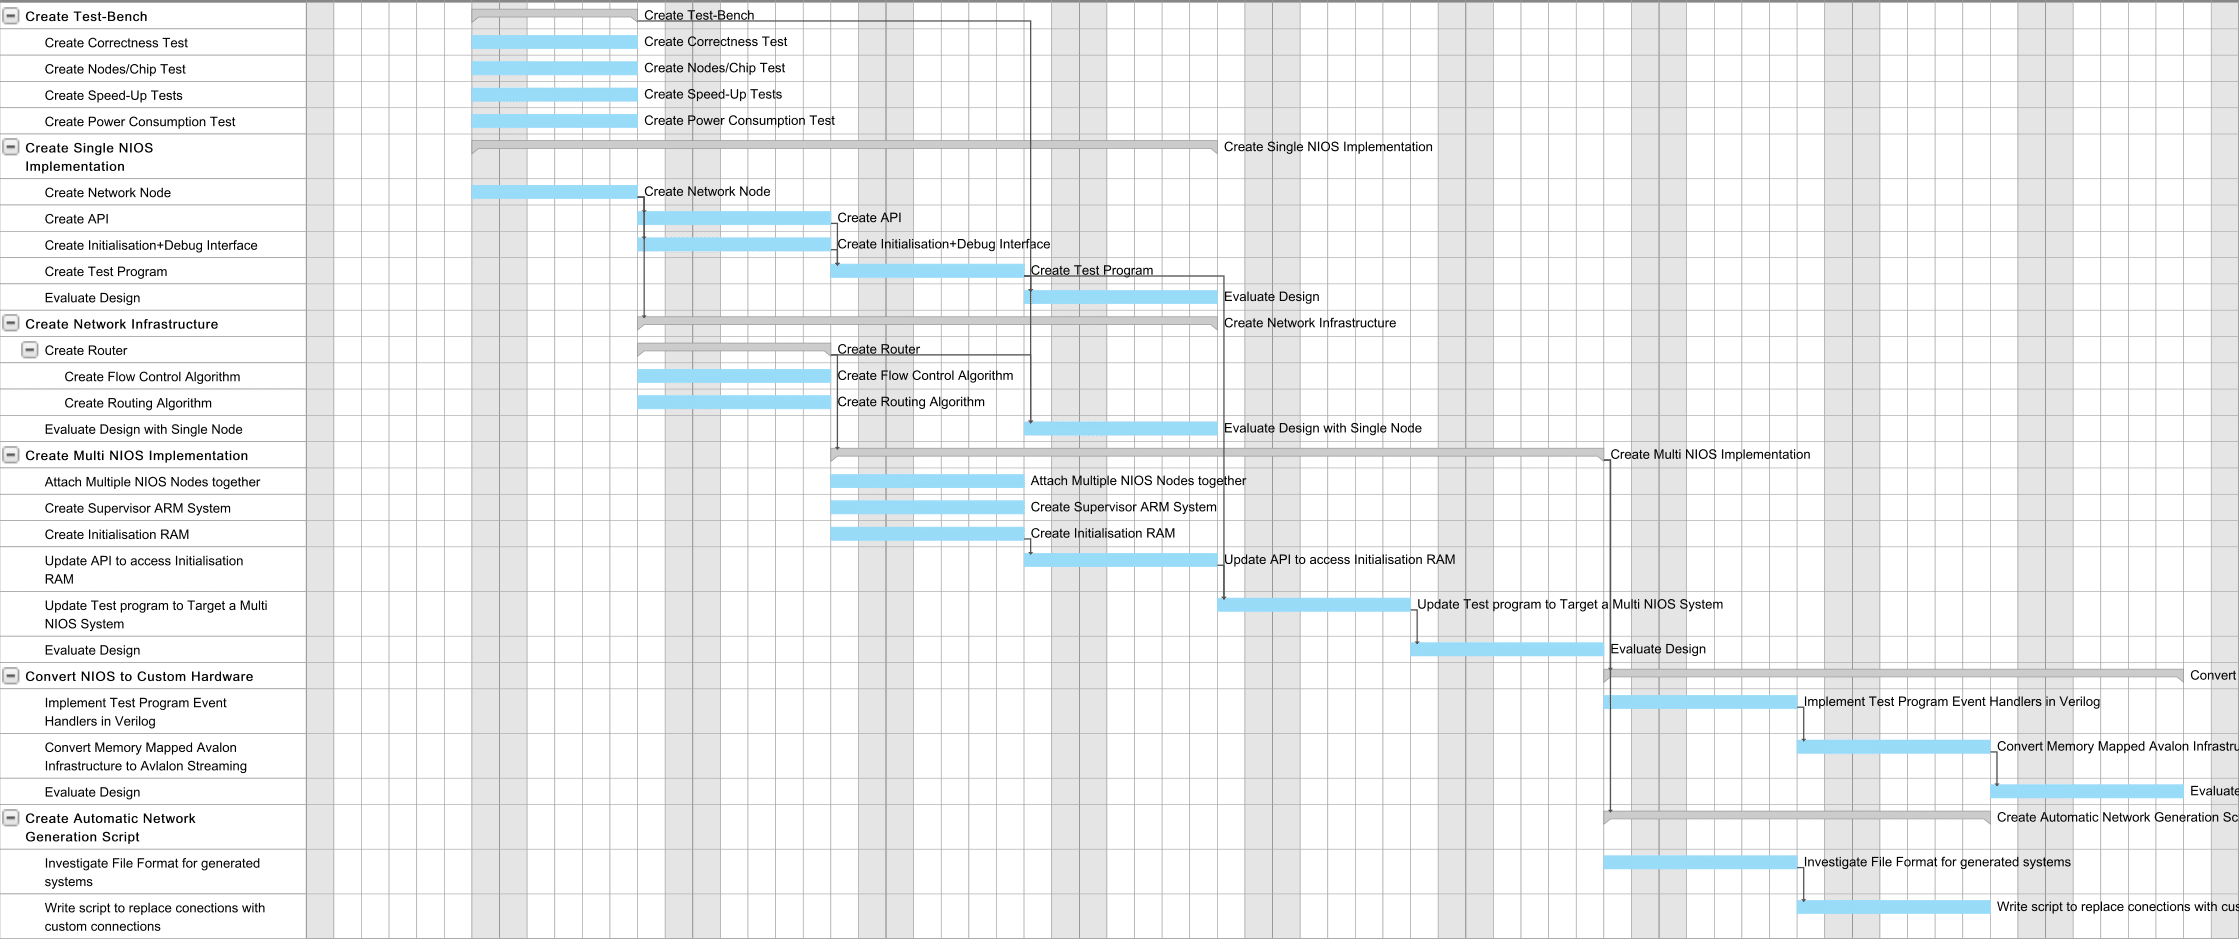
\includegraphics[angle=90,origin=c,height=0.6\textheight]{gantt-1.png}
\caption{Gantt Chart of Milestones and Dependencies}
\label{fig:gantt}
\end{figure}

\subsection{Required Milestones}

These are milestones that must be completed for the project deliverables to be met and the project completed.

\subsubsection{Create Test-bench}

\paragraph{Description}

The first milestone that must be completed is the creation of a test-bench. This will allow the verification of the correctness of the different designs that will be created. This test-bench will run through a specific pattern of tests and provide a short report of the different quantitative criteria that are explained in \cref{subsec:quantitative}. By printing out this report, it will be easier to compare different designs based on the evaluation criteria 

By creating a test-bench to provide quantitative evaluation of my designs, the process will be automated, allowing for a faster evaluation cycle as well as allowing me to perform multiple tasks in parallel instead of requiring a manual setup and execution of every test.

This test-bench will be in the form of a small script or program which executes individually created tests in sequence. The results of these tests may need to be formatted depending on the exact output given and then saved to a file to be used later as a benchmark value for future tests.

\paragraph{Risks}

A major risk with this milestone is the over-complication the test-bench and thus development of it taking up time that is better spent on developing other milestones. As such, vigilance is required to make sure that the minimum time that is needed will spent on this milestone and the over-complication issue is avoided.

In addition, some of the tests are more important than others, especially the correctness test. As such, those tests that are less important or easier to test by hand than by the test-bench (such as number of \glspl{network node} on each \gls{fpga}) are of lower priority and so will have to be removed from the test-bench should it be getting to complicated or taking too long.

\subsubsection{Single \gls{nios}-based \glsentryname{poets} System}

\begin{figure}[h]
\centering
\missingfigure{Missing Single node Poets System}
\caption{Design of a single-node \gls{poets} system}
\label{fig:single_node}
\end{figure}

\paragraph{Description}

The first usable milestone that must be completed is the creation of a single \gls{network node} on the \gls{fpga} which will run a simplified version of the \gls{cpu} based \gls{poets} system. Each of the \glspl{software node} will be run on the same \gls{thread} with all networking between the \glspl{software node} being handled by the software itself.

To complete this milestone, the \gls{poets} system must be simplified to remove the requirements for multiple \glspl{thread} as these are not supported by the \gls{hal}\cite{wiki:hal} and would require a full \gls{os} to be installed, reducing the performance and increasing the memory required to store the program.

In addition, for this milestone to be completed, a single \gls{network node} will have to be designed and implemented as shown in \cref{fig:single_node}, together with the \gls{api} to allow the custom \gls{poets} event handlers to interact with memory and provide the necessary abstraction to allow for easier programming of the \gls{application}. 

\paragraph{Risks}

This milestone relies a working \gls{cpu} based version of the \gls{poets} software as well as a Terasic DE1-SoC board on which it can be tested. If the \gls{poets} software is not available, then this milestone can still be completed, although it may not match the \gls{poets} specification as closely as it would otherwise have.

If the DE1-SoC development board is missing, then parts of the hardware and software can still be developed through the use of simulation but cannot be combined until the board is available. This will mean that development the next milestones will have to begin to keep on schedule but cannot be integrated until everything is tested.

\subsubsection{Network on Chip Infrastructure}

\paragraph{Description}

To create a multi \gls{network node} based system, an important requirement is the networking infrastructure between all of the nodes within a single \gls{fpga}. This infrastructure will transport \glspl{message} between the \glspl{software node} in the form of network \glspl{message} and handle the routing of these \glspl{message} as well as flow control.

This infrastructure has two components that have to be developed to make sure that the result fulfils the criteria given in \cref{subsec:deliverables}. The first component that must be developed and implemented is the router for standard point-to-point routing between \glspl{network node}. In this case, it may be useful to implement a form of default routing like the \gls{spinnaker} uses as shown in \cref{fig:gals_router}. At this, point the performance of different routing algorithms will have to be evaluated to determine which one is the best for this system.

The second component for flow control may be required, depending on the measured throughput of the previously mentioned routing algorithm. If the throughput is too low, then I will have to implement a module into the router that attempts to ease the congestion along a particular \gls{edge}. In essence, this component will have the same purpose as the emergency router in the \gls{gals} system \cite{art:1_plana_furber_temple_khan_shi_wu_yang_2007}. However, it will have to designed slightly differently to fulfil the requirement of no \glspl{message} being dropped. On the other hand, I do not need to account too much about hardware failures as this network will be built onto a single \gls{fpga}.

\paragraph{Risks}

Within this milestone, the development has all been done before and as such is known to be possible. The major risk in doing it though is the risk of missing the internal deadline for this milestone. If it appears to become the case, the first response would be to remove the requirement for flow control from within the network. While it is useful for a fast implementation of the "Multi \glsentryname{nios}-based \glsentryname{poets} System" (\cref{subsec:multi_nios}) milestone, the system will work without it due to the guarantee of no \glspl{message} being list.

Unfortunate

\subsubsection{Multi \glsentryname{nios}-based \glsentryname{poets} System}
\label{subsec:multi_nios}

\begin{figure}[h]
\centering
\missingfigure{Missing Multi node Poets System}
\caption{Design of a multi-node \gls{poets} system}
\label{fig:multi_node}
\end{figure}

\paragraph{Description}

Once I have finished the previous milestones, I am ready to connect multiple \gls{nios} based \glspl{network node} into a single \gls{poets} system within a single \gls{fpga}. This milestone will provide the first working version of a \gls{poets} system on an \gls{fpga} with multiple \glspl{software node} running at the same time and passing \glspl{message} between each other.

While much of the infrastructure to create this milestone will have been done in the previous milestones, at this stage, the software will have to similarly be updated so that it can run on multiple \glspl{software node} at the same time in an asynchronous fashion.

In addition, due to there being multiple \glspl{software node} running at the same time, it will be difficult to oversee all of them and initialise them by hand. As such, a comprehensive initialisation, debugging and data extraction infrastructure will need to be created at this point to allow for the system to automatically be configured to run the application with as little intervention on my part as possible. This system will also allow me to oversee and debug the application much more easily.

To do this, each \gls{software node} will require an interface to expose the internal memory as well as routing configuration to some sort of overseer (most likely the ARM based \gls{cpu} on the \gls{fpga}, although a \gls{soft processor} would also work) which allows for the extraction of debugging information and also initialisation of the \gls{software node}'s memory.

\paragraph{Risks}

\subsection{Optional Milestones}

These are milestones that should be completed by the end of the project but that can be removed if the project falls behind schedule/they are too difficult to complete.

\subsubsection{Replace \glsentryname{nios} with Custom Hardware} \label{subsec:custom_hw}

\paragraph{Description}

Once I have created the basic network for \gls{poets} to run on using \gls{nios} processors, the next task that I will have to complete is to replace the \gls{nios} processors with custom Verilog hardware. This will ideally reduce the complexity of the \glspl{network node} as the \gls{nios} itself uses up around 16000 logic element. In addition, this change will allow me to transition from memory-mapped model to a streaming model, thereby potentially improving the throughput of each node.

To achieve this, I will have to write custom Verilog modules that perform the same actions as the curretn \gls{poets} receive and send event handler have as well as the memory storage for that \gls{software node}'s state. HOwever, the routing system will not have to be modified as the interface between the processing \gls{software node} and the router already had the streaming interface.

\paragraph{Risks}

\subsubsection{Automatic Node Creation Script}

\paragraph{Description}

Another optional milestone that I wish to complete is a script to automatically create and connect the system based on a few input parameters. At small sizes, the system can be built up and connected by hand but after a while, this method becomes unwieldy, especially for the network connections.

As Quartus saves the project in a variant of XML data, it should not be a difficult task to create a parser for this file and insert new \glspl{network node} to it with the correct network connections. By doing this, I will be able to significantly cut dfoen on the time that it will take to generate different sized networks and be able to automate a significant portion of the repetitive work that I will end up doing.

As this will cut down on the work that I will be doing, it may be beneficial to complete this milestone as soon as I have the first working version of the multi-node system in place, but it is not required to complete the project and so will remain an optional milestone.

\paragraph{Risks}

\subsection{Extension Milestones}

These milestones are not expected to be completed unless everything else goes better than expected and the project is already fulfilling all objectives.

\subsubsection{\glsentrylong{hls} for Custom Hardware}

An automation task that would be beneficial for this project is to automate the creation of the event handlers from the C code that it is written in to the verilog that is required for the replacement of \gls{nios} with custom hardware milestone (\cref{subsec:custom_hw}). To reduce the amount of work that I will have to do when converting more complicated programs into verilog.

Doing this will save me some time although it may become very complicated, especially with all of the data structures that \gls{poets} includes as well as the interface to the actual hardware that will have to be considered.

\paragraph{Description}

\paragraph{Risks}

\section{Evaluation Plan}

\subsection{Evaluation Criteria}

\subsubsection{Quantitative}\label{subsec:quantitative}

These criteria are ones that I will use to evaluate the \todo{finish}

To compare these results, I will require a benchmark result which I can use a s baseline to determine how the performance of the tested design has changed. For this I will use a \gls{cpu} based version of the \gls{poets} system as this is for all intents and purposes correct and is also the version of \gls{poets} that I started the project with. However, this version can have wildly different performance characteristics depending on the hardware that it is running on.

To account for this, all of the benchmarks should come from a single hardware configuration to allow for correct comparisons during the evaluation stage. While I could use my personal computer for this test, \gls{poets} is designed to take advantage of a larger numbers of parallel \glspl{cpu}. As such I will attempt to create a benchmark of the \gls{poets} \gls{cpu} application on the hardware that it was originally designed upon at Cambridge University for the BIMPA project\cite{pub:naylor2014rapid}\todo{Maybe explain more} and fall back to my personal computer should this not prove a feasible solution. However, at that point, the results that I will gather for quantitative evaluation will no longer accurately reflect the parallelism that the \gls{poets} system provides.

In either case, it will be beneficial to store the baseline results to prevent changes in result data between individual tests and also considerable speed up the time taken to test any evaluation criterion due to the time taken to recompute the baseline having been removed.

\todo{add flow chart of testing procedure here}

\paragraph{Correctness}

The most important criteria for which I will have to evaluate each solution to my project is correctness. For this, I will have to compare my implemented solution against a reference solution which will be the \gls{cpu} version of \gls{poets}. If the results that are received from both versions are identical for a given test program, then I will know that the solution is correct and can then go on to evaluate the other criteria.

This criteria will ideally be done through a \gls{bit-exact} matching of the reference output and the output of the tested system at each step. As the \gls{poets} architecture only releases the result once all \glspl{software node} have reached the same time step/calculation step, these results should be identical regardless of teh system that they are running on.

During testing with a simulation program running on a \gls{cpu} and later on a \gls{gpu}, I noticed that the results did not always match up in a \gls{bit-exact} pattern. These differences could not easily be predicted beforehand although they tended to be low in number. They also tended to appear more frequently on computational heavy tasks and those where floating point numbers were being used.

There are two main methods to avoid this sort of error during the testing of this project that do not restrict the types of tests that can be run. The first is to manually go over the results every time these errors appear and determine if they are significant or not. This method will obviously be slow to do and also complicated for large scale tests with many results.

The second method that I can apply is to use a simple statistical model to automatically decide whether the errors that were found are true errors or simply due to differences in the hardware that is running the test. For this I could use measures such as the \gls{bit-exact} difference between the two values as well as the total number of errors that have occurred. If both values are less than some to be determined threshold, then the errors can be safely ignored.
\todo{Output type?}

\paragraph{Nodes On Chip}

The main advantage that an \gls{fpga} has over traditional \glspl{cpu} is the ability to have many components in parallel. As such, the number of \glspl{network node} that can be fit on a single \gls{fpga} is an important evaluation criterion. This will allow me to compare different implementations as well as versions of the same implementation to evaluate what provides the best usage of the total area of the \gls{fpga}.\todo{Feels like missing explanation}

For this criterion, the measure will be number of discrete \glspl{network node} that can be placed onto the Cyclone V \gls{fpga} that I am working with, together will all of the associated infrastructure that they require. For this criterion, there is the danger of the tooling optimising the placement of the different designs by different amounts if left to their own devices with the highest possible timing requirements. As such, for this criterion, the timing requirements will be considerably relaxed to allow the tooling to place the design 

In addition, for this criterion, there is the danger that the testing of it can take considerable time as the design will have to be rebuilt with an ever increasing number of \glspl{network node} contained within it. As such, I will have to calculate the maximum number of theoretical \glspl{network node} contained within the system by dividing the total number of \glspl{logic element} by the number of \glspl{logic element} used within a single \gls{network node} as shown in \cref{eq:max_nodes}.

\begin{equation}\label{eq:max_nodes}
N_{max} = \frac{LE_{total}}{LE_{node}}
\end{equation}

\todo{talk about removing some as this is the theoretical max}

As this criterion is not applicable to any \gls{cpu} implementation of the \gls{poets} system, this criterion will be used in comparison between different \gls{fpga} implementations only and so will not have a baseline value which I will compare against.

\paragraph{Speed-up compared to \glsentryname{cpu} implementation}

One important measure of the performance of my \gls{fpga} based system is to compare the time taken to execute a given set of problems using the standard \gls{cpu} implementation to the implementation on the \gls{fpga}. By running this test I can evaluate how many times faster or slower the \gls{fpga} implementation is compared to \gls{cpu} implementation using the formula shown in \cref{eq:speed_up_cpu}.

\begin{equation}
\label{eq:speed_up_cpu}
S = \frac{T_{\gls{fpga}}}{T_{\gls{cpu}}}
\end{equation}

\paragraph{Speed-up compared to other \glsentryname{fpga} implementations}

To evaluate the different implementations of the \gls{fpga} system, I will have to compare them against each other. From the test to evaluate the speed-up against the \gls{cpu} implementation, I will already have all of the raw data available, so this criteria will simply require calculating the speed-up using the formula shown in \cref{eq:speed_up_fpga}

\begin{equation}
\label{eq:speed_up_fpga}
S = \frac{T_{\gls{fpga}_{new}}}{T_{\gls{fpga}_{old}}}
\end{equation}

\paragraph{Power-usage compared to other \glsentrylong{fpga} designs}

In many of the applications, where a distributed systems are used, power usage is a big concern\cite{pub:4_xizhou_feng_rong_ge_cameron} as it directly relates to heat produces and electricity costs, which are magnified by the number of components running at the smae time in distributed systems.

As such, one evaluation criteria is the power consumed by the designs during normal operation. For this, I will have to create a processing intensive and long-running application, which will be run on the design and the power usage profiled.

While it would be nice to compare the power usage between the \gls{fpga} and a \gls{cpu} implementation, due to the difference in hardware, the results will not be in any way meaningful as different hardware configurations will yield different results. As such, I will focus on differences in power usage of the \gls{fpga} designs as they will all be running on the same hardware.

To calculate the power consumption, I will require a baseline of power consumed by the \gls{fpga} when it is not running. This static power, will always exist in some form or another as all unused transistors will be consuming power all of the time\cite{5_gardiner_2008}. However, as all of these calculations will be running on the same hardware, the power consumption will be roughly similar for all tests or at the very least a function of the transistors used. As such, the measured result can be used to evaluate the different algorithms.

As this method can be quite time consuming and complicated to do on an actual \gls{fpga}, I will use the Altera PowerPlay\cite{man:powerplay} for faster estimation of power usage of the different designs and then use actual measurements when the full designs are completed. By using the Altera tool, I will also be able to compare the estimated power usage for different sizes of systems as well.

\paragraph{Maximum Clock Frequency}

For an \gls{fpga}, the maximum clock frequency that the design can run at is a good measure of how well the design works on the \gls{fpga}. With higher clock frequencies meaning that the system is better pipelined. However, much of the performance in this regard comes from how much effort the fitter puts in to try and meet the timing constraints. As such, I will have to take care to have the amount of effort that the tools do for each test to be the same.

One way of doing this is to keep recompiling the system with increasing frequency constraints until it cannot be done. However, this has the downside of taking a very long time to do, especially near the limit of clock frequencies.

As such, a second way would be to compare the estimated maximum clock frequencies that \gls{quartus} reports during compilation. While this measurement is not as exact as the previous method it will suffice for the detection of large changes in this value but will have difficulties with very similar clock frequencies.

\subsubsection{Qualitative}

Some of the evaluation criteria cannot be quantified into any meaningful value. While these are important, they are not as important as the quantitative criteria that the designs exhibit. To evaluate these criteria, I will have to base the results on personal experience and only in a comparative sense, e.g. 'A is easier to use than B' or 'B appears to scale to larger systems compared to A'. The main reason I am basing these on personal experience while developing the project is due to there not being enough time available to train others in the use of the system and then judge their responses.

\paragraph{Ease of Scaling}

The first of qualitative criterion that I will be judging is how the system appears to scale to a larger number of \glspl{software node}. This does not mean how many nodes it can theoretically or practically support as this will be limited by the address space and network congestion. Instead, I will be judging how much effort it takes to create a network of a certain size and then add extra \glspl{software node}.

Actions like placing all connections by hand and individually changing addresses will mean a worse ease of scaling than an automated tool that automatically creates a network for a given input size.

\paragraph{Flexibility of Application}

The second qualitative criterion is how flexible the system is in terms of custom applications. If the developer who is developing on the system requires a lot of effort to produce an application that the system was not explicitly designed for, then the flexibility of it will be rather poor. On the other hand, if the system can easily be used with a wide variety of application types, then the flexibility will be higher.

\section{Conclusion}

\printglossaries

\printbibliography

%%% End document
\end{document}